\subsection{Top Countries and Trends} \label{vizcountries}
 

\begin{figure}
\centering
\fbox{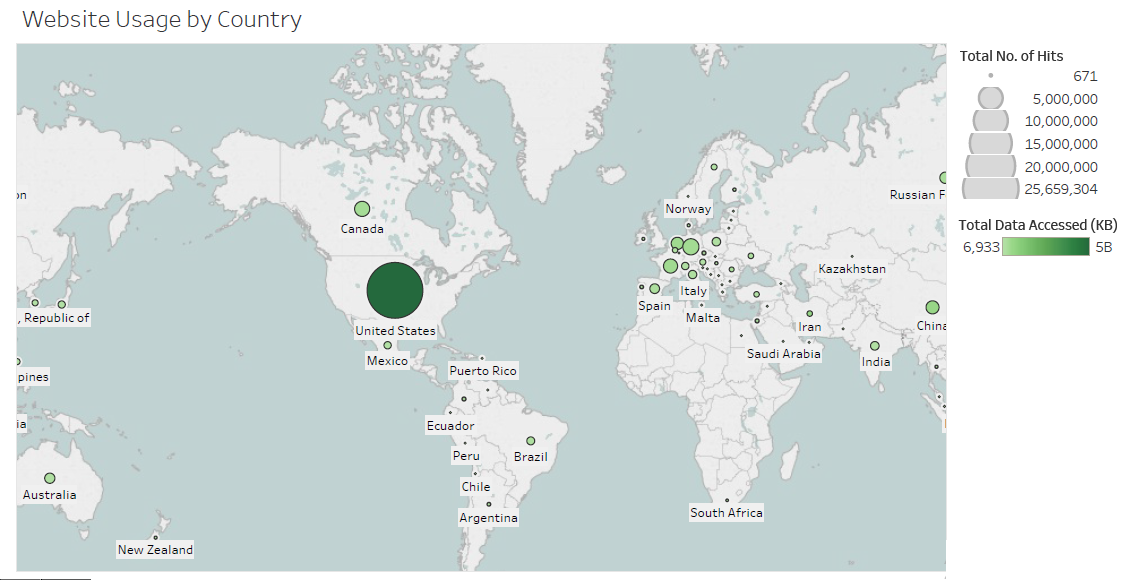
\includegraphics[width=\linewidth]{img/TopCountries2.png}}
\caption{Geospatial Analysis of Web Traffic}
\label{fig:TopCountries}
\end{figure}

Using Tableau, we were able to geocode country names into lattitude and longitude values. We the visualized the same using one of the in-built maps in Tableau. We chose to use the proportional symbol map for this purpose that where the size of the symbol would indicate the number of total hits over a period of timme. Using color we were able to show levels of total data consumed by each of the countries. Users are predominantly from United States but one key insight that was uncovered is that after 2015, proportion of users from countries(e.g. Germany and France ) apart from the US has increased. 
